\documentclass[10pt]{article}

\usepackage[margin=0.75in]{geometry}
\usepackage{amsmath,amsthm,amssymb}
\usepackage{xcolor}
\usepackage{cancel}
\usepackage{graphicx}
\usepackage{changepage}
\usepackage{circuitikz}
\usepackage{pgfplots}
\usepackage{physics}
\usepackage{hyperref}
\usepackage{siunitx}
\usepackage{fontspec}
\usepackage{relsize}
\usepackage{subfig}
\usepackage{todonotes}
\usepackage{minted}
\usepackage{multicol, multirow, booktabs}
\usepackage[breakable]{tcolorbox}
\usepackage[inline]{enumitem}

\theoremstyle{definition}
\newtheorem{problem}{Problem}
\newtheorem{soln}{Solution}

\pgfplotsset{compat=newest}
\usetikzlibrary{lindenmayersystems}
\usetikzlibrary{arrows}
\usetikzlibrary{calc}
\usetikzlibrary{positioning, fit}
\usetikzlibrary{3d, perspective}

\definecolor{incolor}{HTML}{303F9F}
\definecolor{outcolor}{HTML}{D84315}
\definecolor{cellborder}{HTML}{CFCFCF}
\definecolor{cellbackground}{HTML}{F7F7F7}
\newcommand{\ui}{\hat{i}}
\newcommand{\uj}{\hat{j}}
\newcommand{\uk}{\hat{k}}
\newcommand{\ux}{\hat{x}}
\newcommand{\uy}{\hat{y}}
\newcommand{\uz}{\hat{z}}
\newcommand{\primed}[1]{#1^\prime}
\pgfdeclarelayer{background}  
\pgfsetlayers{background,main}
\AtBeginDocument{\RenewCommandCopy\qty\SI}

\makeatletter
\newcommand{\boxspacing}{\kern\kvtcb@left@rule\kern\kvtcb@boxsep}
\makeatother
\newcommand{\prompt}[4]{
    \ttfamily\llap{{\color{#2}[#3]:\hspace{3pt}#4}}\vspace{-\baselineskip}
}

\newcommand{\thevenin}[2]{
  \begin{center}
    \begin{circuitikz} \draw
      (0,0) -- (2,0) to[battery1, l_=$V_{Th}\eq#1$] (2,2) 
      to[resistor, l_=$R_{Th}\eq#2$] (0,2)
      ;
      \draw [o-] (-.07,2.079);
      \draw [o-] (-.07,0.079);
    \end{circuitikz}
  \end{center}
}

\newcommand{\norton}[2]{
  \begin{center}
    \begin{circuitikz} \draw
      (0,0) -- (3,0) to[american current source, l_=$I_{N}\eq#1$] (3,2) -- (0,2) (2,0)
      to[resistor, l=$R_{N}\eq#2$] (2,2)
      ;
      \draw [o-] (-.07,2.079);
      \draw [o-] (-.07,0.079);
    \end{circuitikz}
  \end{center}
}

\newcommand{\highlight}[1]{\colorbox{yellow}{$\displaystyle #1$}}

\newcommand{\ti}[1]{\widetilde{#1}}

\newfontface{\Kaufmann}{Kaufmann}
\DeclareTextFontCommand{\kf}{\Kaufmann}
\newcommand{\scriptr}{\fontsize{12pt}{12pt}\kf{r}}

\newfontface{\KaufmannB}{Kaufmann Bd BT}
\DeclareTextFontCommand{\kfb}{\KaufmannB}
\newcommand{\bscriptr}{\fontsize{12pt}{12pt}\kfb{r}}

\newcommand{\bv}[1]{\mathbf{#1}}

\title{Physics 3610H: Assignment IV}
\author{Jeremy Favro (0805980) \\ Trent University, Peterborough, ON, Canada}
\date{\today}

\begin{document}
\maketitle

% PROBLEM 1
\begin{problem}
In class we found the general form of the wavefunction in each region of a finite well to
be
$$
\psi(x)=
  \begin{cases}
    x<-a   & De^{+\kappa x}       \\
    -a<x<a & A\cos kx + B \sin kx \\
    x> a   & Ce^{-\kappa x}       \\
  \end{cases}
$$
Using the continuity of the wavefunction and its first derivative at both $x = -a$ and $x = +a$,
we arrived at the following four equations.
\begin{align}
  \psi(-a)                     & =A\cos ka - B \sin ka  = De^{-\kappa a}          \\
  \psi(+a)                     & =A\cos ka + B \sin ka  = Ce^{-\kappa a}          \\
  \eval{\frac{d\psi}{dx}}_{-a} & = kA\sin ka +kB\cos ka = D\kappa e^{-\kappa a}   \\
  \eval{\frac{d\psi}{dx}}_{+a} & = -kA\sin ka +kB\cos ka = -C\kappa e^{-\kappa a}
\end{align}
Together with normalization these determine $A$, $B$, $C$, $D$ and $E$. In particular, by considering
$(2)-(4)/\kappa$ and $(3)+(5)/\kappa$ we showed that
$$
  A\left(1-\frac{k}{\kappa}\tan ka\right) = B\left(\tan ka + \frac{k}{\kappa}\right)=0
$$
In class we considered the even solutions by setting $B = 0$. Here, consider the odd solutions
by setting $A = 0$.
\begin{enumerate}[label=(\alph*)]
  \item What two equations connect $k$ and $\kappa$ in this case?
  \item Let $x \equiv  ka$ and $y \equiv \kappa a$ and plot both functions on a single plot for $2mV_oa^2/\hbar^2$ = 25.
  \item How many allowed values of energy are there in this case?
  \item Give an approximate value of $\kappa a$ which is allowed.
  \item Use $(1)+(3)/\kappa$ and $(2)-(4)/\kappa$ to determine the values of $C$ and $D$, and write the form of
        the odd wavefunctions in each region in terms of $B$, $k$ and $\kappa$.
\end{enumerate}
\end{problem}
\newpage
\begin{soln}~
  \begin{enumerate}[label=(\alph*)]
    \item We have $$A\left(1-\frac{k}{\kappa}\tan ka\right)=0\implies 1-\frac{k}{\kappa}\tan ka=0\implies k\tan ka = \kappa$$
          and
          $$k^2+\kappa^2 = 2mV_oa^2/\hbar^2.$$
    \item With our previous two expressions relating $k$ and $\kappa$ this gets us
          $$y=-\frac{x}{\tan x}\quad\text{and}\quad y=\sqrt{25-x^2}.$$
          which are plotted in red and blue respectively in the plot below.
          \begin{center}
            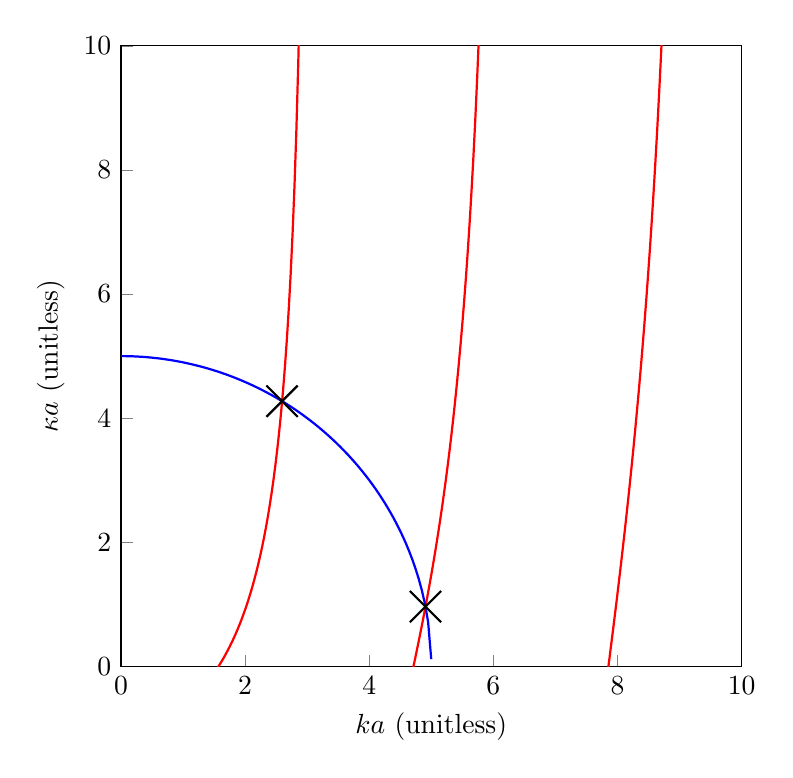
\begin{tikzpicture}
              \begin{axis}[title = {},
                  ymax = 10,
                  ymin = 0,
                  xmin=0,
                  xmax=10,
                  xtick pos = bottom,
                  ytick pos = left,
                  height=0.65\textwidth,
                  width=0.65\textwidth,
                  scale only axis=true,
                  xlabel=$ka$ (unitless),
                  ylabel=$\kappa a$ (unitless),
                  legend pos=north east
                ]
                \draw[red, thick, domain=0.001:{1*pi - 0.1}, samples=100] plot (\x, {
                    -\x/(tan(\x*180/pi))
                  });
                \draw[red, thick, domain={1*pi + 0.1}:{2*pi - 0.1}, samples=100] plot (\x, {
                    -\x/(tan(\x*180/pi))
                  });
                \draw[red, thick, domain={2*pi + 0.1}:{3*pi - 0.1}, samples=100] plot (\x, {
                    -\x/(tan(\x*180/pi))
                  });
                \draw[blue, thick, domain={0}:{5}, samples=100] plot (\x, {
                    sqrt(25-\x^2)
                  });
                \addplot [only marks, mark=x, mark size=8, thick] table {
                    4.906295150856183 0.963466601746654
                    2.5957390796498125 4.27342235572148
                  };
              \end{axis}
            \end{tikzpicture}
          \end{center}
          Points of intersection were found using SageMath after first plotting to determine approximate intervals for a
          numerical solution
          \begin{tcolorbox}[breakable, size=fbox, boxrule=1pt, pad at break*=1mm,colback=cellbackground, colframe=cellborder]
            \prompt{In}{incolor}{1}{\boxspacing}
            \begin{minted}[breaklines, autogobble]{sage}
                x = var('x')

                f(x) = - x / tan(x)
                f1(x) = sqrt(25 - x^2)

                r1 = find_root(f1-f, 0, 3)
                r2 = find_root(f1-f, 3, 5)

                show((r1, f(r1)))
                show((r2, f(r2)))
              \end{minted}
          \end{tcolorbox}
          \begin{tcolorbox}[breakable, size=fbox, boxrule=.5pt, pad at break*=1mm, opacityfill=0]
            \prompt{Out}{outcolor}{1}{\boxspacing}
            $\displaystyle \left(2.5957390796498125, 4.27342235572148\right)$\\
            $\displaystyle \left(4.906295150856183, 0.963466601746654\right)$
          \end{tcolorbox}
    \item Two, as indicated by the plot in the previous part which is a representation of values of
          $E$, the only parameter which is changing in the function, which give consistent $\kappa a$ values.
    \item The two values here are $\approx4.27$ and $\approx0.96$, determined as above using SageMath.
    \item With $A=0$ the equations first simplify to
          \begin{align}
            \psi(-a)                     & =- B \sin ka  = De^{-\kappa a}         \\
            \psi(+a)                     & =+ B \sin ka  = Ce^{-\kappa a}         \\
            \eval{\frac{d\psi}{dx}}_{-a} & = +kB\cos ka = D\kappa e^{-\kappa a}   \\
            \eval{\frac{d\psi}{dx}}_{+a} & = +kB\cos ka = -C\kappa e^{-\kappa a}.
          \end{align}
          Which gives
          \begin{align*}
            (5)+(7)/\kappa \implies & - B \sin ka+\frac{kB}{\kappa}\cos ka  = De^{-\kappa a} + De^{-\kappa a}  \\
            \implies                & B\left(-\sin ka+\frac{k}{\kappa}\cos ka\right)  = 2De^{-\kappa a}        \\
            \implies                & D = \frac{B}{2}e^{\kappa a}\left(-\sin ka+\frac{k}{\kappa}\cos ka\right)
          \end{align*}
          and
          \begin{align*}
            (6)-(8)/\kappa \implies & B \sin ka-\frac{kB}{\kappa}\cos ka = Ce^{-\kappa a}+C e^{-\kappa a}      \\
            \implies                & B \left(\sin ka-\frac{k}{\kappa}\cos ka\right) = 2Ce^{-\kappa a}         \\
            \implies                & C = \frac{B}{2} e^{\kappa a} \left(\sin ka-\frac{k}{\kappa}\cos ka\right)
          \end{align*}
          % Now applying $(5)+(7)/k$,
          % \begin{align*}
          %            & - \frac{B}{k} \sin ka+B\cos ka               = \frac{D}{k}e^{-\kappa a}+\frac{D\kappa}{k} e^{-\kappa a} \\
          %   \implies & B\left(- \frac{1}{k} \sin ka+\cos ka\right)  = \frac{D}{k}e^{-\kappa a}\left(1+\kappa\right)            \\
          %   \implies & D = Be^{\kappa a}\left(1+\kappa\right)^{-1}\left(- \sin ka+k\cos ka\right)
          % \end{align*}
          % and $(6)-(8)/\kappa$
          % \begin{align*}
          %            & \frac{B}{\kappa} \sin ka - \frac{kB}{\kappa}\cos ka = \frac{C}{\kappa}e^{-\kappa a} + C e^{-\kappa a} \\
          %   \implies & \frac{B}{\kappa} \left(\sin ka - k\cos ka\right)     =  Ce^{-\kappa a}\left(1+\frac{1}{\kappa}\right) \\
          %   \implies & C = Be^{\kappa a}\left(1+\kappa\right)^{-1} \left(\sin ka - k\cos ka\right).
          % \end{align*}
          % These are our values for $C(B, \kappa, k)$ and $D(B, \kappa, k)$. $B$ can be determined through normalization.
  \end{enumerate}
\end{soln}
\end{document}